%Schriftgröße, Layout, Papierformat, Art des Dokumentes
\documentclass[footsepline,11pt,oneside,a4paper]{scrartcl}

\usepackage[left=2cm,right=2cm,top=2cm,bottom=2cm]{geometry}
%\usepackage{scrpage2}
\usepackage{fancyhdr} %Paket laden
%mathem. funktionen
\usepackage{amsmath}
\usepackage{listings}
\usepackage{xcolor}
%\usepackage{inconsolata}
\usepackage{amsfonts}
\usepackage{amssymb}
%Umlaute ermöglichen
\usepackage[utf8]{inputenc}
%alte Rechtschreibung
\usepackage{german}
\usepackage{makeidx}
\usepackage{graphicx}
%\usepackage[backend]{graphicx}
\usepackage{color}
\usepackage{units}
\usepackage{latexsym}
\usepackage[final]{pdfpages}
\usepackage{float}
\author{M.Meese/T.Fromme}
\title{Dokumentation Stereoskopie/StereoGL}

\usepackage[T1]{fontenc}
\newcommand{\changefont}[3]{
\fontfamily{#1} \fontseries{#2} \fontshape{#3} \selectfont}

\setlength{\headheight}{2cm}
%\setlength{\footheight}{1cm}
 %\setlength{\footskip}{10mm}
\pagestyle{fancy} %eigener Seitenstil
{%
\fancyhf{} %alle Kopf- und Fußzeilenfelder bereinigen
\fancyhead[]{
\includegraphics[scale=1, width=\textwidth]{img/eps/fhlogo-gd.eps}} %zentrierte Kopfzeile
\fancyfoot[L]{M.Meese/T.Fromme} %Namen
\fancyfoot[C]{Dokumentation Stereoskopie} %Seitennummer
\fancyfoot[R]{\thepage} %Seitennummer
\renewcommand{\headrulewidth}{0.0pt} %obere Trennlinie
\renewcommand{\footrulewidth}{0.4pt} %untere Trennlinie
%\renewcommand{\footskip}{2.4pt} %untere Trennlinie
%\renewcommand{\headskip}{2.4pt} %untere Trennlinie
}%

\lstset{
	language=C,
	backgroundcolor=\color{gray!10},
	breaklines=true,
	inputencoding=latin1
}


\begin{document}
\pagestyle{plain}
\vspace{10cm}
\begin{center}

\includegraphics[scale=1.5,width=1\textwidth]{img/eps/fhlogo.eps} 
\end{center}
\title{\hfill\\Stereoskopie in der grafischen Datenverarbeitung }
\vspace{8cm}
\author{%
	\begin{tabular}[c]{rl}
		Michael Meese & Mat. Nr. : 206549 \\
		Thomas Fromme & Mat. Nr. : 206650 \\
	\end{tabular}
}
\vspace{80pt}
\date{%
	\begin{tabular}[c]{rl}
		 &  \\
		Dokumentationsausarbeitung vom : & 10. August 2012 \\
	\end{tabular}
}
\newpage
\renewcommand{\titlepagestyle}{fancy}
\maketitle
\newpage
%\pagestyle{fancy}
\pagestyle{fancy} %eigener Seitenstil
{%
\fancyhf{} %alle Kopf- und Fußzeilenfelder bereinigen
\fancyhead[]{
\includegraphics[scale=1, width=\textwidth]{img/eps/fhlogo-gd.eps}} %zentrierte Kopfzeile
\fancyfoot[L]{M.Meese/T.Fromme} %Namen
\fancyfoot[C]{Dokumentation Stereoskopie} %Seitennummer
\fancyfoot[R]{\thepage} %Seitennummer
\renewcommand{\headrulewidth}{0.0pt} %obere Trennlinie
\renewcommand{\footrulewidth}{0.4pt} %untere Trennlinie
%\renewcommand{\footskip}{2.4pt} %untere Trennlinie
%\renewcommand{\headskip}{2.4pt} %untere Trennlinie
}%
\changefont{ppl}{m}{n}
\tableofcontents
\listoffigures

\newpage
\section{Konzept und Geschichte der Stereobilderzeugung}

Um räumlich sehen zu können verfügt der Mensch über zwei Augen. Dieses räumliche sehen der Umwelt begeisterte schon im Mittelalter Maler und Gelehrte wie Leonardo da Vinci, die versuchten Tiefeninformationen in ihren Gemälden zu vermitteln, in dem sie versuchten 3Dimensional zu zeichnen. Jedoch enthalten diese Gemälde keine wirkliche Tiefeninformation, da es sich hierbei nur um so genannte Flachbilder handelt, welche dem Betrachter für jedes Auge die gleiche Perspektive liefern. Eine Tiefeninformation wird hier nur angedeutet, da das Gemälde vom Zeichner so angefertigt wurde, dass es eine Vorstellung der räumlichen Perspektive wieder gibt. Aus solchen konventionellen zweidimensionalen Bildern / Gemälden können im Nachhinein also keinerlei Tiefeninformationen mathematisch rekonstruiert werden. Das gleiche gilt auch für Photographien die mit herkömmlichen Kameras angefertigt werden. Diese verfügen nur über ein Objektiv, was vergleichbar wäre mit einem Menschen der ein Auge zu kneift [HERBIG]. Für die Wahrnehmung eines räumlichen Bildes ist es also zwingend notwendig, jedem Auge des Betrachters eine spezifische Perspektive der zu visualisierenden Szene darzubieten. Dies ist mittels Stereoskopischer Techniken realisierbar. Man spricht von so genannten Stereobildern. 
\vspace{1.0cm}
\begin{figure}[h]
  \centering
  
		\includegraphics[scale=0.8]{img/ps/wahrnehmung.eps} 
				\caption{Prinzip der Wahrnehmung}
				\label{Prinzip der Wahrnehmung}

\end{figure}
\newpage

Der Begriff „Stereoskopie“ setzt sich aus den zwei griechischen Wörtern stereo (räumlich) und skopein (sehen) zusammen. Es handelt sich hierbei um ein Verfahren bei dem paarweise Bilder (stereoskopische Halbbilder genannt) getrennt für jedes Auge angeboten werden. Die darzustellenden Raumpunkte sind durch korrespondierende Bildpunkte auf jedem Halbbild abgebildet. Aufgrund der Parallaxe sind diese ein wenig seitenverschoben zueinander (genannt: stereoskopische Deviation). Unter der sogenannten Deviation versteht man den horizontalen Abstand gleicher Bildelemente auf beiden Halbbildern zueinander. Die Deviation ist damit die Abbildung der Parallaxe [WikiStereo]. Das Prinzip der Stereoskopie ist demnach ganz einfach. Der Mensch sieht die Welt mit zwei Augen, wobei jedes Auge die Welt aus einer anderen Perspektive wahrnimmt. Durch das binokulare (beidäugige) Sehen ist es dem Mensch möglich, die Welt in drei Dimensionen wahrzunehmen. Das Gehirn verarbeitet die Halbbilder dann zu einem dreidimensionalen Abbild. Die Stereoskopie setzt bei der Zuführung der Bildinformationen an das jeweilige Auge an. Ziel ist es, wie bei dem natürlichen Sehvorgang die Augen jeweils mit einem für sie perspektivisch korrekten Bild zu versorgen. Vergleicht man stereoskopische Bilder mit herkömmlichen 2D-Bildern, so ist der wohl größte Vorteil der Stereoskopie sofort erkennbar. Es wird dem Betrachter ermöglicht, die Lage der abgebildeten Raumpunkte zu empfinden. Dies ist letztendlich auf die Repräsentation der Bilddaten zurück zu führen, da diese dem natürlichen Sehvorgang sehr nahe kommt. 
\vspace{1cm}

Der englische Physiker Charles Wheatstone (1802-1875) gilt als der Urvater der Stereoskopie. Im Jahr 1832 hatte er bereits zwei Modelle nach seinen angaben anfertigen lassen. Anschließend erschienen 1833 Informationen über seine Experimente in der dritten Auflage der Outlines of Human Physiology. Kurz vor der Veröffentlichung der Photographie teilte er 1838 seine Erkenntnisse der Royal Society in London mit. Bereits hier verwies er auf diverse Betrachtungsgeräte. Im gleichen Jahr noch veröffentlichte Wheatstone am King’s College London, seine ersten Forschungsergebnisse über räumliches Sehen. Er berechnete und zeichnete Stereobildpaare und konstruierte für deren Betrachtung einen Apparat, bei dem der Blick des Betrachters durch Spiegel auf die Halbbilder umgelenkt wurde (siehe Abbildung 1). Diesen Apparat nannte er Stereoskop [Stereo]. 
\vspace{0.5cm}

\begin{figure}[h]
  \centering
		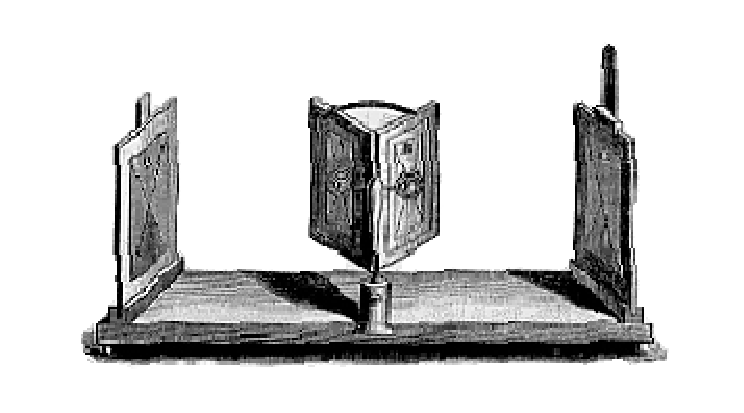
\includegraphics[scale=1,width=\textwidth]{img/gif/Spiegelstereoskop.eps} 
		\caption{altes Spiegelstereoskop}
		\label{altes Spiegelstereoskop}
\end{figure}
\newpage

\begin{figure}[h]
  \centering
		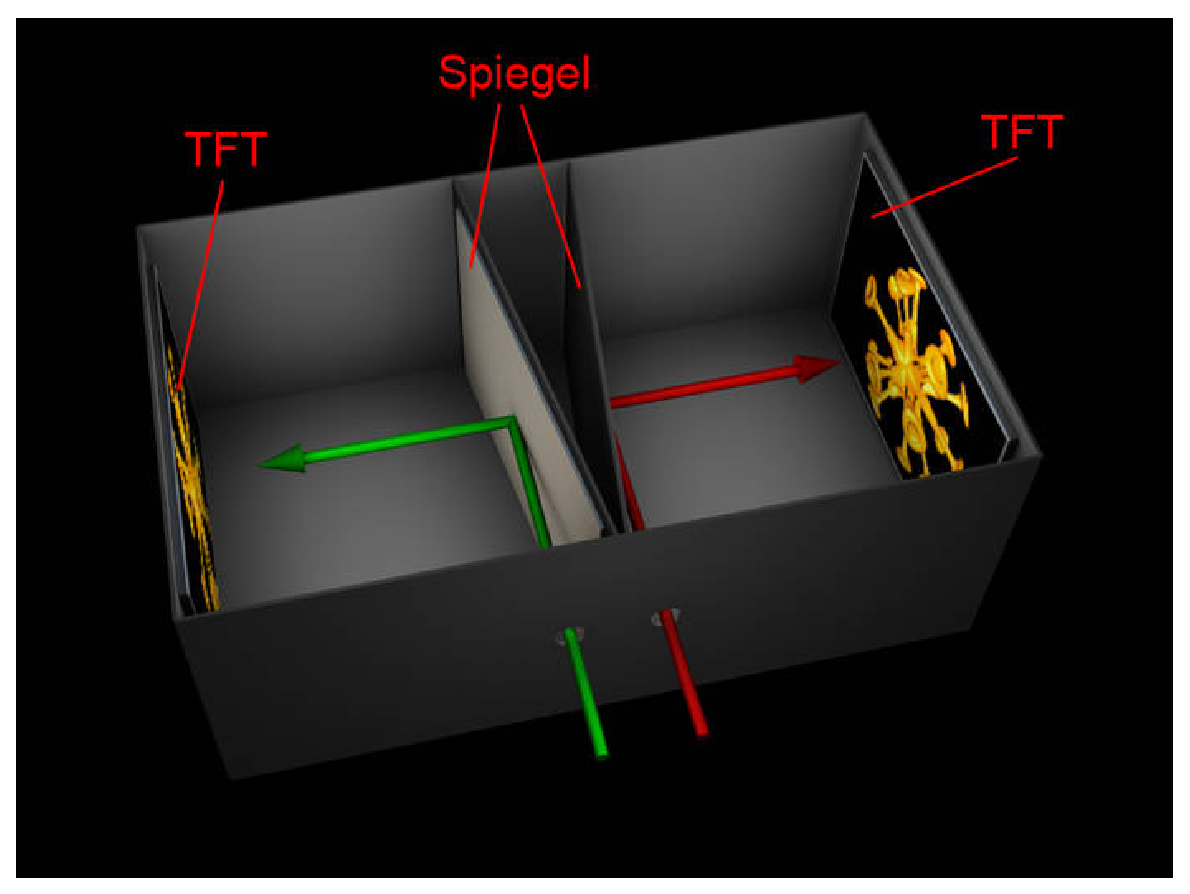
\includegraphics[scale=0.5,width=0.8\textwidth]{img/ps/Spiegelstereoskop2.eps} 
		\caption{Spiegelstereoskop}
		\label{Spiegelstereoskop}
\end{figure}
\vspace{2cm}

\section{Parallaxen bei stereoskopischen Bildern}
Parallaxe entscheiden über die Wahrnehmung der Objekte im Bezug auf die dritte Dimension. Es existieren drei verschiedene Arten von Parallaxen. Hierbei handelt es sich um die so genannte „Null Parallaxe“, die „Negative Parallaxe“, sowie die „Positive Parallaxe“.

\vspace{2cm}
\subsection{Null Parallaxe}
Die homologen Bildpunkte beider Bilder liegen bei der Null Parallaxe genau übereinander. Bei der Betrachtung eines Bildpunktes mit Null-Parallaxe,schneiden sich die optischen Achsen in der Ebene der Leinwand (siehe Abbildung 4).
\vspace{1cm}
\begin{figure}[h]
  \centering
		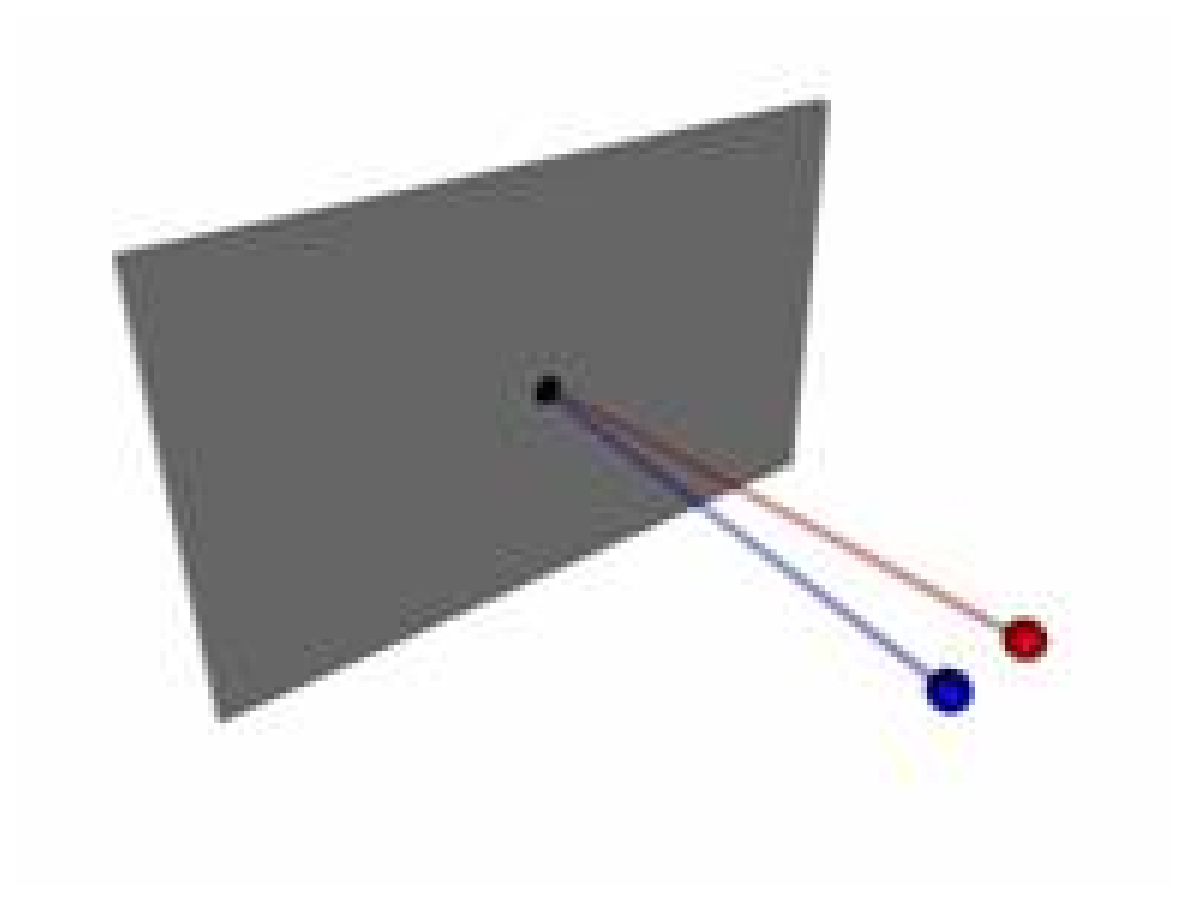
\includegraphics[scale=1,width=0.5\textwidth]{img/new/Null-Parallaxe.eps} 
		\caption{Null-Parallaxe}
		\label{Null-Parallaxe}
\end{figure}

\vspace{2cm}
\subsection{Positive Parallaxe}
Bei einer positiven Parallaxe entspricht der Wert der Parallaxe dem Augabstand. Eine parallele Ausrichtung der optischen Achse beider Augen ist der Fall. Wahrzunehmen ist diese, bei der Betrachtung von Objekten in sehr großer Ferne (siehe Abbildung 5).
Sämtliche Objekte, welche sich hinter der Projektionswand oder gar nicht schneiden erzeugen Bilder, welche hinter der Projektionswand wahrgenommen werden.
\vspace{1cm}
\begin{figure}[h]
  \centering
		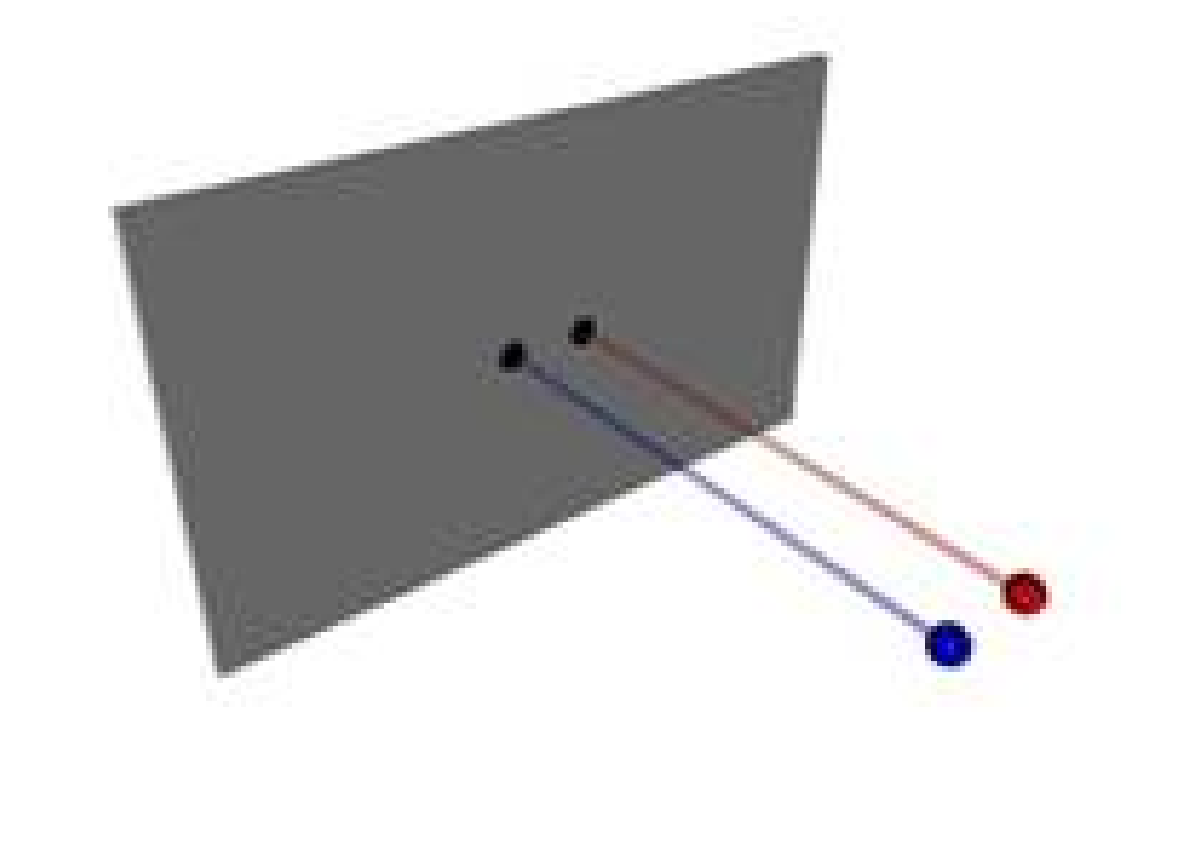
\includegraphics[scale=1,width=0.5\textwidth]{img/new/PositiveParallaxe.eps} 
		\caption{Positive Parallaxe}
		\label{Positive Parallaxe}
\end{figure}

\newpage
\subsection{Negative Parallaxe}
Bei einer negativen Parallaxe, kreuzen sich die optischen Achsen vor der Bildschirm Ebene. Die Objekte werde so also hervorragend wahrgenommen (siehe Abbildung 6).
\vspace{1cm}
\begin{figure}[h]
  \centering
		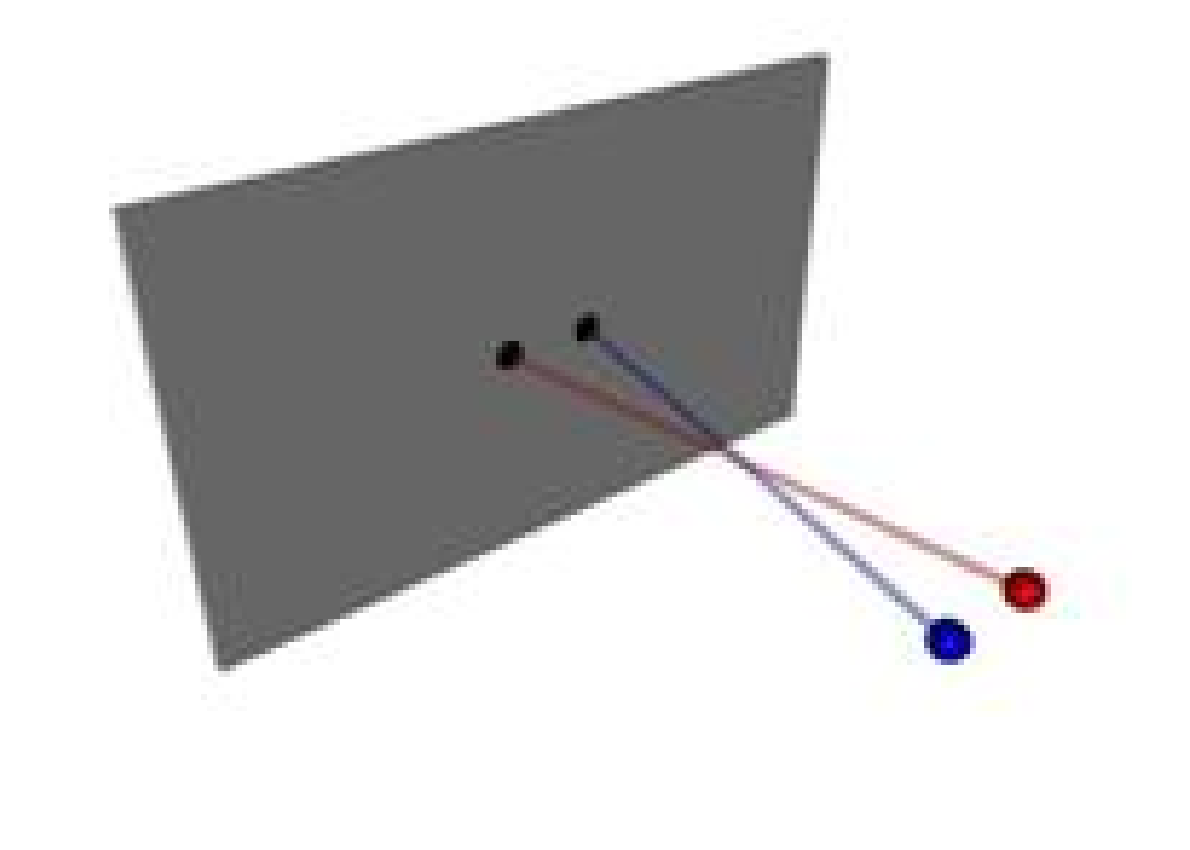
\includegraphics[scale=1,width=0.5\textwidth]{img/new/NegativeParallaxe.eps} 
		\caption{Negative Parallaxe}
		\label{Negative Parallaxe}
\end{figure}

\vspace{2cm}
\begin{figure}[h]
  \centering
		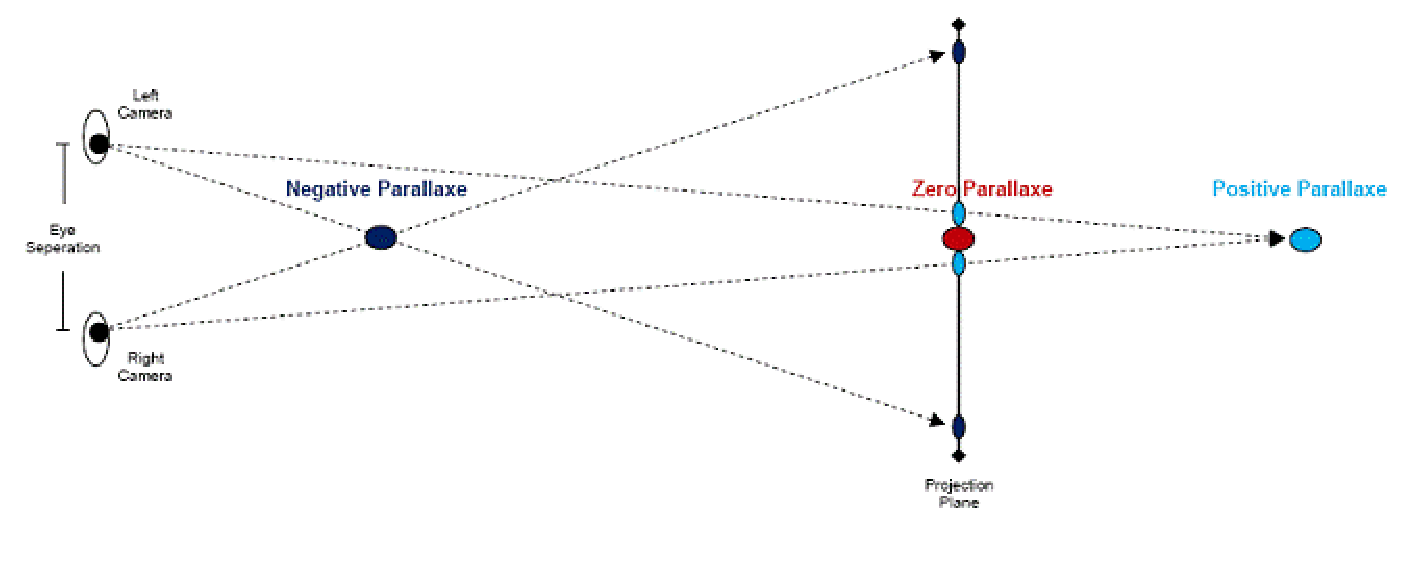
\includegraphics[scale=1,width=1\textwidth]{img/alleParallaxe.eps} 
		\caption{Negative Parallaxe}
		\label{Negative Parallaxe}
\end{figure}
\newpage
\section{Stereoskopische Verfahren}
\vspace{1cm}
Die heutigen sechs etablierten Verfahren der Stereoskopischen Darstellung sind:
\vspace{0.5cm}
\begin{tabbing}
\hspace{10pt}\=\kill
\textbullet \>Infitec\\
\textbullet \>Anaglyphen\\
\textbullet \>Autostereoskopisches verfahren\\
\textbullet \>Polarisationstechnik\\
\textbullet \>Shuttertechnik\\
\end{tabbing}

\vspace{1cm}

\subsection{Infitec}
Infitec ist ein Verfahren  welches eine Kanaltrennung bei Stereoprojektionen basierend auf Interferenzfiltern vorsieht. Durch verschiedenfarbige Filter werden Farben für das menschliche Auge ausgeblendet und somit entsteht ein räumlicher Effekt wenn diese im Kopf wieder zusammengesetzt werden
\vspace{2cm}
\begin{figure}[h]
  \centering
		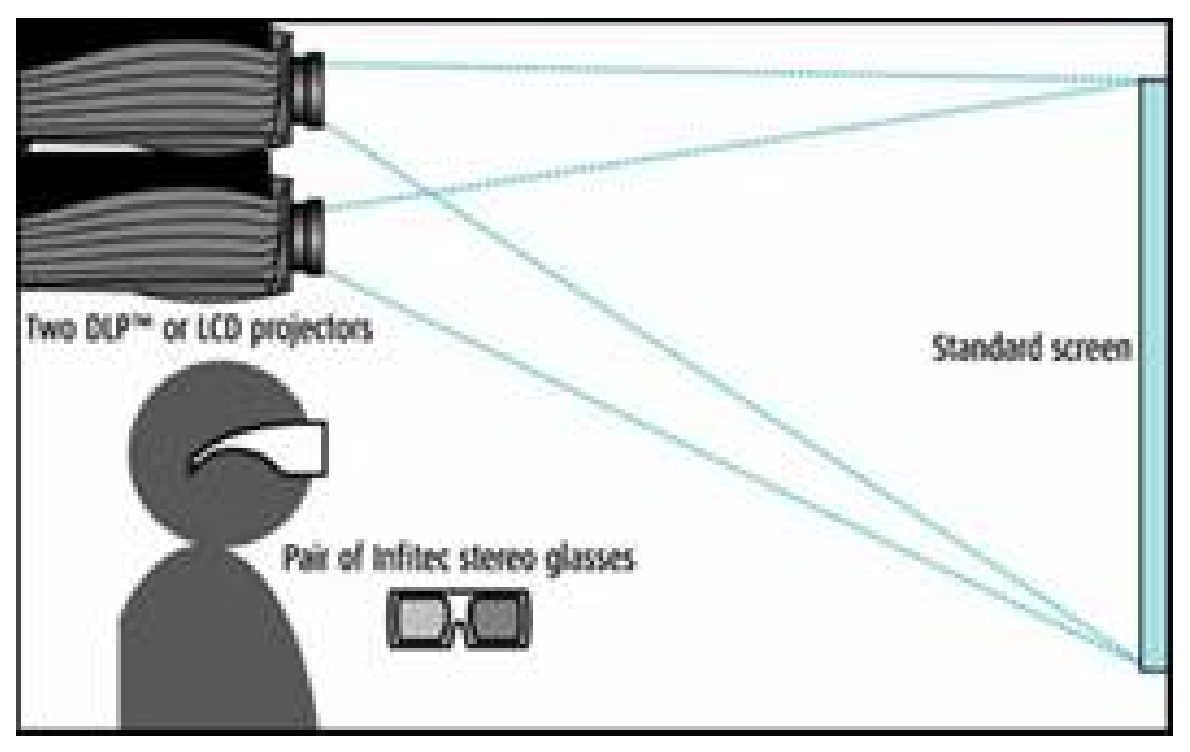
\includegraphics[scale=0.5,width=0.5\textwidth]{img/new/InfitecSystemaufbau.eps} 
		\caption{Infitec Systemaufbau}
		\label{Infitec Systemaufbau}
\end{figure}
\vspace{1cm}
\newpage
\subsection{Anaglyphen}
Es handelt sich hierbei um das wohl populärste und verbreitetste Verfahren der Stereoskopie. Hierbei werden Halbbilder komplementär [Farbimp] einzufärben und anschließend übereinander zu legen [Anaglyph].
\vspace{2cm}
\begin{figure}[h]
  \centering
		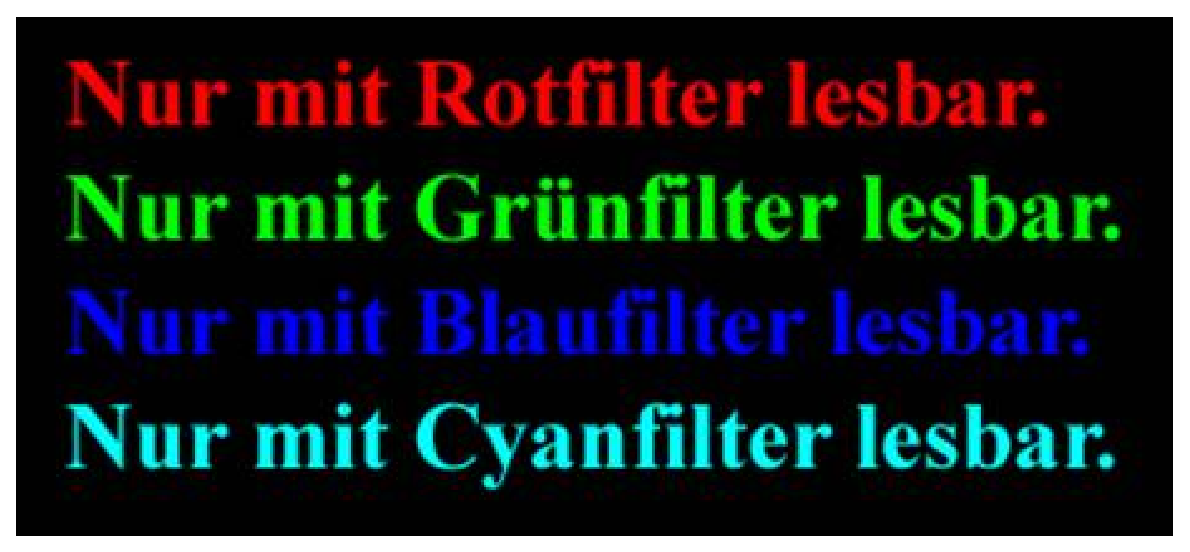
\includegraphics[scale=0.5,width=0.5\textwidth]{img/new/FarbfilterTest.eps} 
		\caption{Farbfilter Test}
		\label{Farbfilter Test}
\end{figure}
\vspace{1cm}
\subsection{Autostereoskopisches verfahren}
Die Autostereoskopie ist ein Verfahren, bei dem man dreidimensionale Bilder mit Tiefeneindruck darstellt, ohne dass der Benutzer auf Betrachtungsgeräte zurückgreifen muss. Hierbei werden keine Brillen mehr benötigt.

\vspace{2cm}
\begin{figure}[h]
  \centering
		\includegraphics[scale=0.8,width=0.8\textwidth]{img/new/autostereoskopischenDisplays.eps} 
		\caption{autostereoskopische Displays}
		\label{autostereoskopische Displays}
\end{figure}

\newpage
\subsection{Polarisationstechnik}
Die Polarisationsfiltertechnik ist  ein sehr weit verbreitetes Projektionsverfahren, welches nicht nur zu wissenschaftlichen Zwecken, sondern auch bei 3D - Filmen in den heutigen Kinos eingesetzt wird (z.B. IMAX oder Real D).

\vspace{2cm}
\begin{figure}[h]
  \centering
		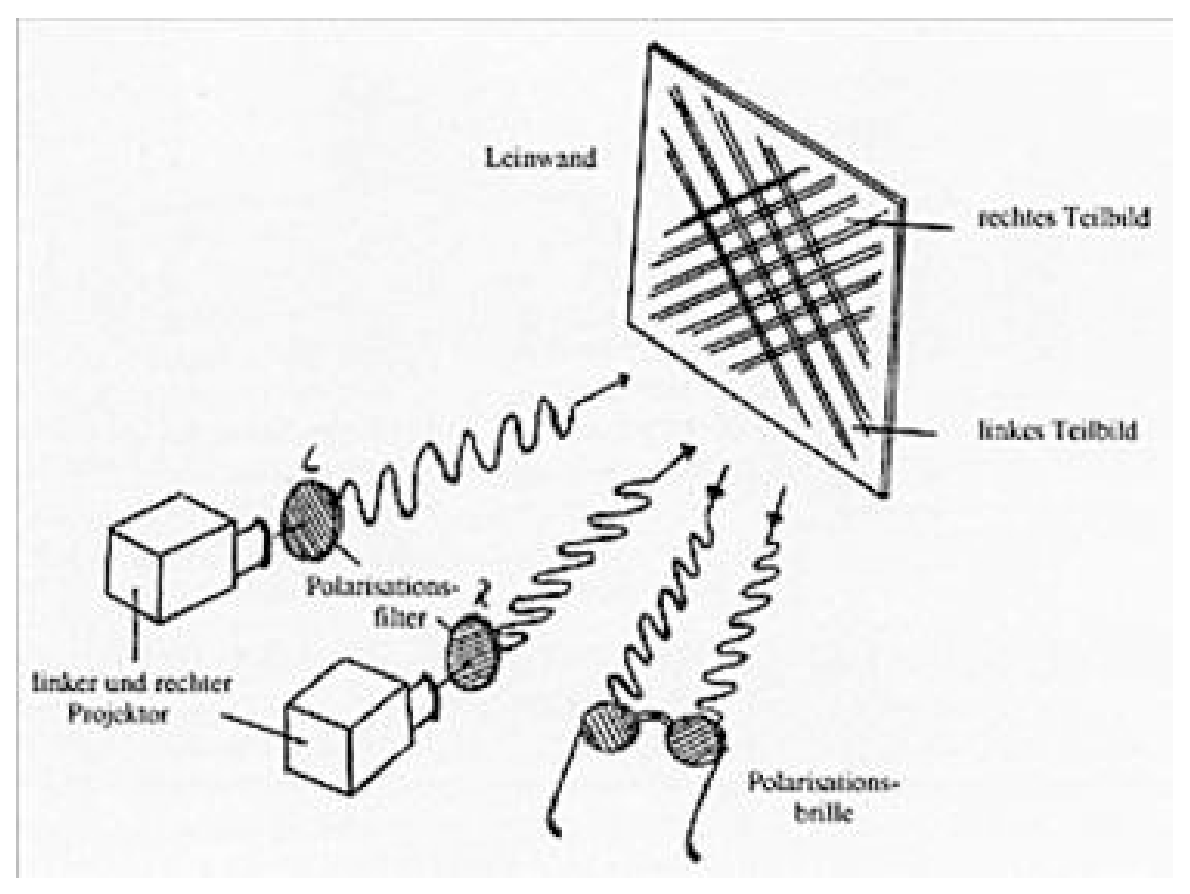
\includegraphics[scale=0.8,width=0.8\textwidth]{img/new/Polarisationsfiltertechnik.eps} 
		\caption{Polarisationsfiltertechnik}
		\label{Polarisationsfiltertechnik}
\end{figure}

\newpage
\subsection{Shuttertechnik}
Bei diesem Verfahren werden nacheinander Halbbilder bei 60 Bildern / Sekunde projeziert. Durch einen Infrarot Signalgeber, werden die sogenannten Shutterbrillen mit dem Film synchronisiert.




\vspace{1cm}
\section{Stereoskopie mit OpenGL }
\vspace{1cm}
\subsection{Das Programm}
Im folgenden werden relevante Teile des Sourcecodes erklärt. Der vollständige Sorucecode befindet sich im Anhang dieser Dokumentation.
\vspace{0.5cm}
Da die Entwicklung des Programms hauptsächlich unter Linux erfolgte, das fertige Programm aber ebenfalls unter Windows lauffähig sein sollte, wurde die plattformunabhängige Library SFML (Quelle http://www.sfml-dev.org/) genutzt. Dies ermöglichte eine Portierung des Programms ohne größeren Aufwand.
\vspace{0.5cm}
Die SFML Library stellt die Schnittstelle zum Betriebssystem her und sorgt für die Ein- und Ausgabe des Bildes bzw. die Entgegennahme der Steuerbefehle von der Tastatur. Ebenfalls entfällt das Einbinden der OpenGL-Librarys, da SFML dies für den Entwickler übernimmt. Die OpenGL-Librarys GLU und GLUT müssen nicht desto trotz auf dem Entwicklungssystem vorhanden sein.
Vorweggreifend kann gesagt werden, dass das Programm ohne Anpassungen auf Windows kompiliert werden konnte. Lediglich die SFML-Library musste dem Compiler bekannt gemacht werden.
\newpage
Entwickelt wurde das Programm auf einem Ubuntu Linux 10.04.4 LTS 64Bit. Als Compiler kam der gcc in der Version 4.4 zum Einsatz. Die OpenGL Librarys wurden in Form des Metapaketes libglu1-mesa-dev (Quelle Webseite der libmesa) in der Version 7.7.1 verwendet. Die mesa Library liefert in einem Paket alle benötigten OpenGL Librarys mit. Die SFML Library lag in der Version 1.5 vor.
\vspace{2cm}
\subsection{Darstellungslisten}
Die ersten Versionen des Programms wurden ohne Darstellungslisten umgesetzt. Die jeweiligen OpenGL-Anweisungen wurden prozedural Schritt für Schritt aufgerufen. Durch das Hinzufügen einzelner Elemente des Hauses, entwickelte der Code langsam eine ungünstigte „Spaghetti“ Struktur. Die weitere Entwicklung wurde Schritt für Schritt komplizierter.
\vspace{0.5cm}
Die Umstellung auf Darstellungslisten erhöhte ungemein die Lesbar- und Wartbarkeit des Codes. Das Haus konnte dadurch wie ein Fertigbauhaus in einzelnen Elementen erstellt und später Schritt für Schritt via Aufruf „zusammengebaut“ werden. So konnten später auch leichter Elemente verändert oder hinzugefügt werden.

\subsubsection{Verwendung von Listen}
Um Darstellungslisten zu verwenden, werden im ersten Schritt Listennamen angelegt. Eine Listenname ist in OpenGL eine Ganzzahl vom Datentyp GLint. 
\vspace{1cm}


\begin{lstlisting}
    [caption={Verwendung von Listen}\label{lst:code01},captionpos=t] 
// Listendefinitionen
// 0-9 Hauptlisten
#define SZENE				1 // Gesamte Szene
// 10-999 Unterlisten
#define KOORDINATENSYSTEM		10
#define RASEN				20
#define HAUS				30
	#define WAENDE			310
	#define DACH			320
	#define DACHGIEBEL		330
	#define DACHFLAECHEN		340 // Ziegelflaechen
	#define SCHORNSTEIN		350
	#define HAUSTUER			360
	#define FENSTER			370
	#define DREMPEL			380
   #define BAEUME				40
	#define KRONE			410
	#define STAMM			420
   #define GAUBE				50
	#define GWAENDE			510
	#define GDACH			520

 \end{lstlisting}

 
Um eine gewisse logische Struktur zur erhalten, wurde das Haus in die eben schon erwähnten Fertighaus Komponeten zerlegt und in absteigender Abhängigkeit definiert.
%\vspace{2cm}
 \newpage
\subsubsection{Listen generieren}
Eine neue Liste wird mit dem Befehl $glNewList$ angelegt. Als Paramter werden der Listenname und  der Paramter für den Listengenerierungsmodus.$ GL_COMPILE $sorgt dafür, dass der enthaltene Code kompiliert und zum späteren Aufruf vorgehalten wird.
\vspace{0.5cm}
Die Liste selbst enthält dann weitere OpenGL Befehle, die in diesem Fall die Primitive $GL_QUADS$ enthält. In diesem Fall werden die beiden Dachflächen für die Gaube gezeichnet.
\vspace{1cm}
\begin{lstlisting}
    [caption={Listen generieren}\label{lst:code02},captionpos=t] 
// Dach der Gaube zeichnen
glNewList((GLint) GDACH, GL_COMPILE);
	glEnable(GL_TEXTURE_2D);
	glBindTexture(GL_TEXTURE_2D, textures.Dach);
	glBegin(GL_QUADS);
		// Flaeche Dach rechts
		glColor3f(1, 1, 1);
		glNormal3f(0.706298, 0.707914 , 0);
		glTexCoord2f(0, 0); glVertex3f(v28[0]-5, v28[1], v28[2]);
		glTexCoord2f(0, 1); glVertex3fv(v29);
		glTexCoord2f(1, 1); glVertex3f(v23[0]-5, v23[1]-5, v23[2]+5.5);
		glTexCoord2f(1, 0); glVertex3f(v24[0]-5, v24[1]-5, v24[2]+5.5);
		// Flaeche Dach links - Gelb
		glColor3f(1, 1, 1);
		glNormal3f(-0.706298, 0.707914 , 0);
		glTexCoord2f(0, 0); glVertex3f(v28[0]-5, v28[1], v28[2]);
		glTexCoord2f(0, 1); glVertex3fv(v29);
		glTexCoord2f(1, 1); glVertex3f(v26[0]-5, v26[1]-5, v26[2]-5.5);
		glTexCoord2f(1, 0); glVertex3f(v27[0]-5, v27[1]-5, v27[2]-5.5);
	glEnd();
	glDisable(GL_TEXTURE_2D);
glEndList();

 \end{lstlisting}

\newpage
\subsubsection{Verschachtelung von Listen}
Listen können auch verschachtelt werden. Heißt, das eine Liste eine vorher definierte Liste einfach nur aufruft, aber keine neuen OpenGL Elemente enthält. Diese Möglichkeit wurde genutzt und logische Bauteile zu erstellen und somit leichter lesbare Struktur in den Quelltext zu bringen.
\vspace{1cm}

\begin{lstlisting}
    [caption={Verschachtelung von Listen }\label{lst:code03},captionpos=t] 
// Gaube
glNewList((GLint) GAUBE, GL_COMPILE);
	glCallList((GLint) GWAENDE);
	glCallList((GLint) GDACH);
glEndList();

 \end{lstlisting}

\vspace{0.5cm}
In diesem Beispiel wird die Liste GAUBE erstellt, welche die vorher definierten Listen GWAENDE und das vorherige Beispiel GDACH aufruft.
\vspace{0.5cm}
Zum Schluss wird dann mit der gleichen Technik die Liste SZENE erstellt, welche alle Listen der zu zeichnenden Szene enthält.
\vspace{1cm}
\begin{lstlisting}
    [caption={Verschachtelung von Listen 2}\label{lst:code04},captionpos=t] 
glNewList((GLint) SZENE, GL_COMPILE);
	glScaled(zoom,zoom,zoom); // Szene zoomen
	glCallList((GLint) HAUS);
	glCallList((GLint) BAEUME);
	glCallList((GLint) RASEN);
glEndList();

 \end{lstlisting}
\vspace{0.5cm}

Abschließend wird dann nur noch die Liste SZENE aufgerufen und damit alle vorherigen Listen aufgerufen und gezeichnet.
\vspace{0.5cm}
\vspace{1cm}
\begin{lstlisting}
    [caption={Szene }\label{lst:code05},captionpos=t] 
glCallList((GLint) SZENE);
 \end{lstlisting}

\vspace{0.5cm}

\newpage
\subsection{Zwei parallele Views}
Von der Umsetzung eher trivial, aber für die parallele Darstellung von zwei leicht unterschiedlichen Motiven sinnvoll, ist die Erstellung von zwei Views. Der View ist im Prinzip der Bereich in dem die OpenGL Szene gezeichnet wird.
\vspace{0.5cm}
Normalerweise wird deswegen nur ein View erstellt, welcher die OpenGL Szene enthält. Zunächst wurde dieser Weg beschritten, in dem das Objekt zweimal mit einem Offset auf der X-Achse gezeichnet wurde. In der weiteren Entwicklung stellte sich aber heraus, das es ziemlich umständlich wurde beide Objekte unabhängig von einander zu steuern und den generellen Offset der Rotation um die Y-Achse zu realisieren. 
\vspace{0.5cm}
Mit zwei unabhängigen Views wird die zu zeichnende Szene zweimal erstellt aber mit unterschiedlichen Parametern initialisiert.
\vspace{0.5cm}
\vspace{1cm}
\begin{lstlisting}
    [caption={Zwei parallele Views }\label{lst:code06},captionpos=t] 

for(i=0; i<2; i++){
	if (i == 0) {
		// Linker Viewport
		glLoadIdentity();
		glTranslatef(0.f, 0.f, -200.f);
		glRotated(140, 0, 1, 0); // Szene um 45° zur Y-Achse drehen.
		glRotatef(rotx, 0.f, 1.f, 0.f); // Szene um die Y-Achse drehen
		glRotatef(roty, 1.f, 0.f, 0.f); // Szene um die X-Achse drehen
		glViewport(view0.x, view0.y, view0.w, view0.h); // linker Viewport
		}
		// Rechter Viewport
	else if (i == 1) {
		glLoadIdentity();
		glTranslatef(0.f, 0.f, -200.f);
		glRotated(140, 0, 1, 0); // Szene um 45° zur Y-Achse drehen.
		// Szene unabhaengig um die Y-Achse drehen
		glRotated(stereoy, 0, 1, 0);
		// Szene unabhaengig um die X-Achse drehen
		glRotated(stereox, 1, 0, 0); 
		glRotatef(rotx, 0.f, 1.f, 0.f); // Szene um die Y-Achse drehen
		glRotatef(roty, 1.f, 0.f, 0.f); // Szene um die X-Achse drehen
		glViewport(view1.x, view1.y, view1.w, view1.h); // rechter Viewport
		}
	glCallList((GLint) SZENE);
}
 \end{lstlisting}

\newpage
Der Befehl $glViewport(view0.x, view0.y, view0.w, view0.h)$ lädt den Viewport mit den Koordinaten für den linken Viewport und $glViewport(view1.x, view1.y, view1.w, view1.h);$ den rechten.
\vspace{1cm}
\begin{lstlisting}
    [caption={Viewport views }\label{lst:code07},captionpos=t] 
const int width = 1200;
const int height = 600;

Viewport view0 = { 0, 0, width / 2 - 1, height - 1 };
Viewport view1 = { width / 2, 0, width / 2 - 1, height - 1 };

 \end{lstlisting}
\vspace{0.5cm}
Ein Viewport wird mittels X/Y/Z-Koordinaten. In diesem Fall wird ein Offset über die gesamte Größe des Fensters errechnet und in den Structs view0 und view1 abgelegt. Im obigen Beispiel greift glViewport dann auf diese Structs zu.
\vspace{2cm}
\subsection{Rotation}
Um den 3D-Effekt zu erzielen, wie weiter oben in den Kapiteln über die Stereoskopie beschrieben, muss das Objekt in einem Viewport unter einem anderem Betrachtungswinkel dargestellt werden. Da wie oben beschrieben zwei Viewports verwendet werden, ist dies mit einer Zeile erledigt.
\vspace{1cm}
\begin{lstlisting}
    [caption={Rotation}\label{lst:code08},captionpos=t] 
    
float stereoy = 3; // mit 3° Offset um die Y-Achse drehen

glRotated(stereoy, 0, 1, 0); // Szene um die Y-Achse drehen
 \end{lstlisting}

\vspace{0.5cm}
Der erste Parameter von $glRotated $ gibt den Winkel in Grad vom Datentyp $ GLdouble$ an, um den gedreht werden soll. Die weiteren Parameter werden ebenfalls als $GLdouble$ angegeben und repräsentieren die jeweilige X/Y/Z-Achse um die gedreht werden soll. Im obigen Beispiel sind die X- und die Y-Achse mit einer 0 deaktiviert. Somit erfolgt eine Drehung nur um die Y-Achse um den Wert von $stereoy$.
\newpage
\subsection{Bedienung}
Da der 3D-Eindruck abhängig von der Größe und Auflösung des jeweiligen Monitors ist, bietet das Programm folgende Justagemöglichkeiten:

	\vspace{2.5cm}
	\begin{tabular}{|l|c|}
	\hline 
	Funktion & Tasten \\ 
	\hline
	  &   \\ 
	\hline  
	gleichzeitige Rotation beider Views um X- und Y-Achse & Pfeiltasten \\ 
	\hline 
	Rotation des rechten Views um die X- und Y-Achse & W/AS/D \\ 
	\hline 
	Reset der Rotation des rechten Views & R \\ 
	\hline 
	Zoom der Szene In und Out & Z/U \\ 
	\hline 
	\end{tabular} 
\vspace*{3.5cm}

\vspace{0.5cm}
Die Steuerung erfolgt ausschließlich über die Tastatur, da bewusst auf Steuermöglichkeiten in Form einer GUI verzichtet wurde.
\vspace{0.5cm}
Da sich der Benutzer nach unserer Erfahrung ausschließlich auf die Fokussierung des Bildes konzentrieren muss, kann während der Betrachtung nicht der Blickpunkt auf Elemente in der GUI verlegt werden. Aus diesem Grund ist eine „blinde“ Bedienung über die Tastatur sinnvoll.

\newpage
\section{Quellen:}
Bei der Erstellung wurde auf folgende Quellen zurückgegriffen:
\vspace{1cm}
\begin{tabbing}
\hspace{10pt}\=\kill
\textbullet \>Jetzt lerne ich OpenGL ISBN: 3-8272-6237-2\\
\textbullet \>http://wiki.delphigl.com/index.php/Hauptseite\\
\textbullet \>http://www.sfml-dev.org/tutorials/1.5/window-opengl.php\\
\textbullet \>Wikipedia Stereoskopie\\
\textbullet \>Grundlagen der Stereoskopie der Hochschule Darmstadt
\end{tabbing}
\vspace{2cm}


\end{document}